% !TEX root = ../thesis.tex
\chapter{Methodology}
	\label{chap:typesetting}
	In order to apply any ML and NLP to the tweet dataset, to see if we could do any information extraction and statistical analysis, we first needed to be able to generate a ranking of the ten tweets we had obtained. We sourced the tweets themed around Brexit on Twitter, and then a pipeline (see fig: \ref{fig:pipeline}) for sourcing peoples preferences of the tweets was created. The pipeline created was handled by the web app. The web app allowed the user to create an account and then compare the tweets. The resulting decision updated the ELO rating for each tweet and the more simplified traditional comparison judgment method. Each user gets only presented five different combinations, ensuring that a single tweet was only seen by the user once.
	
	\begin{figure}[t]
		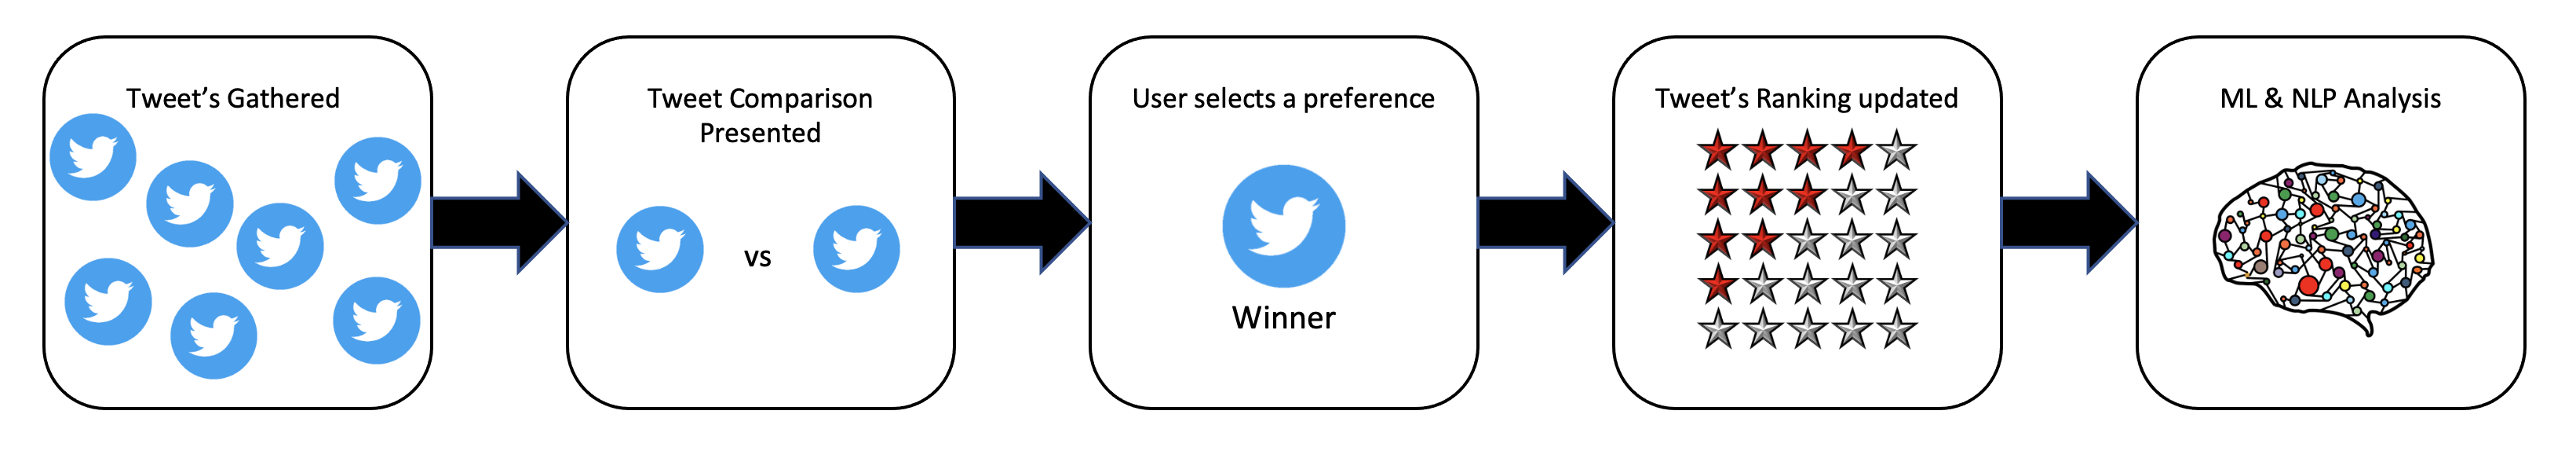
\includegraphics[width=\textwidth]{pipline.png}
		\caption{A visual representation of the processes pipline.}
		\label{fig:pipeline}
		
	\end{figure}
	
	\section{Tools}
	To create the web application and insights from the tweets, we required to use several tools. It is a requirement that we develop a full-stack web application with a user UI, an area to input the user's judgements on the tweet, store the results using a database, and extract information from the tweets using NLP techniques. Several factors within the final application needed to be satisfied for the tools to be appropriate for use.
	
	
	\subsection{Programming Language}
	While many programming languages can handle creating a full-stack application and conducting ML, for example, Java, Php and JavaScript. We decided to use the Python language. We decided upon Python due to our familiarity with it over the other main languages and its versatility. We made this decision because Python can make full-stack applications with the use of additional libraries and handle most NLP ML tasks using libraries like NLTK, SpaCy, Sci-Kit Learn, and TensorFlow.
	
	\subsection{Libraries}
	\subsubsection{Web Application}
	For creating the web application, there were two main libraries available. These were Django and Flask.
	
	Django is a high-level Python Web framework that encourages rapid development and clean, pragmatic design. Built by experienced developers, it takes care of much of the hassle of Web development, so you can focus on writing your app without needing to reinvent the wheel. It’s free and open source \cite{django}.
	
	While Flask is a small framework by most standards—small enough to be called a “micro- framework,” and small enough that once you become familiar with it, you will likely be able to read and understand all of its source code \cite{grinberg2018flask}. 
	
	Flask has three main dependencies. The routing, debugging, and Web Server Gateway Interface (WSGI) subsystems come from Werkzeug; the template support is provided by Jinja2; and the command-line integration comes from Click. These dependencies are all authored by Armin Ronacher, the author of Flask \cite{grinberg2018flask}. 
	
	Flask has no native support for accessing databases, validating web forms, authenti‐ cating users, or other high-level tasks. These and many other key services most web applications need are available through extensions that integrate with the core pack‐ ages. As a developer, you have the power to cherry-pick the extensions that work best for your project, or even write your own if you feel inclined to. This is in contrast with a larger framework, where most choices have been made for you and are hard or sometimes impossible to change \cite{grinberg2018flask}.
	
	%decision and justification
	After experimenting with the two frameworks, we decided upon Flask. Flask got decided upon because of the short time frame to put the project together. Additionally, the lightweight nature of the framework also played a fact. As this will be just an initial prototype, Django's other requirements would be unessential additionals to the project. Therefore, taking focus away from what we believe is the main focus. 
	
	\subsubsection{NLP Tasks}
	
	
	
	\subsection{IDE}
	While many great IDEs are available like Pycharm, Jupyter Lab, Atom and Sublime, we decided to use VS Code. The decision behind this was that it allowed us to explore code within interactive python notebooks (ipynb) and standard python scripts. Additionally, it allowed us to create HTML, CSS, and Javascript files within the same IDE.
	
	\section{Software Development Life Cycle Methodology}
	Agile [ref from previous msc?]
	
	
	
	\section{Ranking System}
	
	As discussed in the literature review, along with a more traditional pairwise comparative judgment algorithm, we could choose either an ELO or Glicko system. While each has advantages and disadvantages, we decided to use the ELO system. We decided to use this system as we felt it would be more robust for how we intend to be calculating the tweet scores, as we will be taking random pairings of tweets that will only be seen once by the user. The user only seeing the tweet appear once removes any opportunity for a user to underrate a tweet because it has been seen multiple times and not lose its impact on the user. 
	
	Due to this reason, the ELO system, with its probability aspect to the scoring, helped determine outcomes on potential unseen tweet combos. While not considering if a tweet gets seen more than any others, this would have a massive impact on the comparative judgement pairwise comparison method.
	
	
	\begin{figure}[t]
		\centering
		 Prob A Wins$ = 1/1+10^{(B-A/400)}$
		\caption{To calculate the expected score for a tweet.}
		\label{fig:elo_maths_1}
	\end{figure}

\begin{figure}[t]
	\centering

	new score $= rating + 32 * $  score $ - $ expected score
	\caption{A visual representation of the web apps navigation.}
	\label{fig:elo_maths_2}
\end{figure}
	
	\section{Data Set}
	
	\subsection{Data Capture Method}
	
	\subsection{Pre-Processing}
	
	
	\section{Implementation}
	%[gather tweets]
	
	%[Web App]
	The web application got implemented using the Python web library Flask. The web application used several industry-standard tools, for example, HTML, CSS, JavaScript, Bootstrap and dynamic content. The HTML, CSS, Bootstrap and JavaScipt was used to handle the application's front end. The web application had a mesh style navigation system (see fig: \ref{fig:web_app_nav}). However, when the user was on the compare page, this would push to itself and update the users content based on what they had next in their comparison list.
	
	\begin{figure}[t]
		\centering
		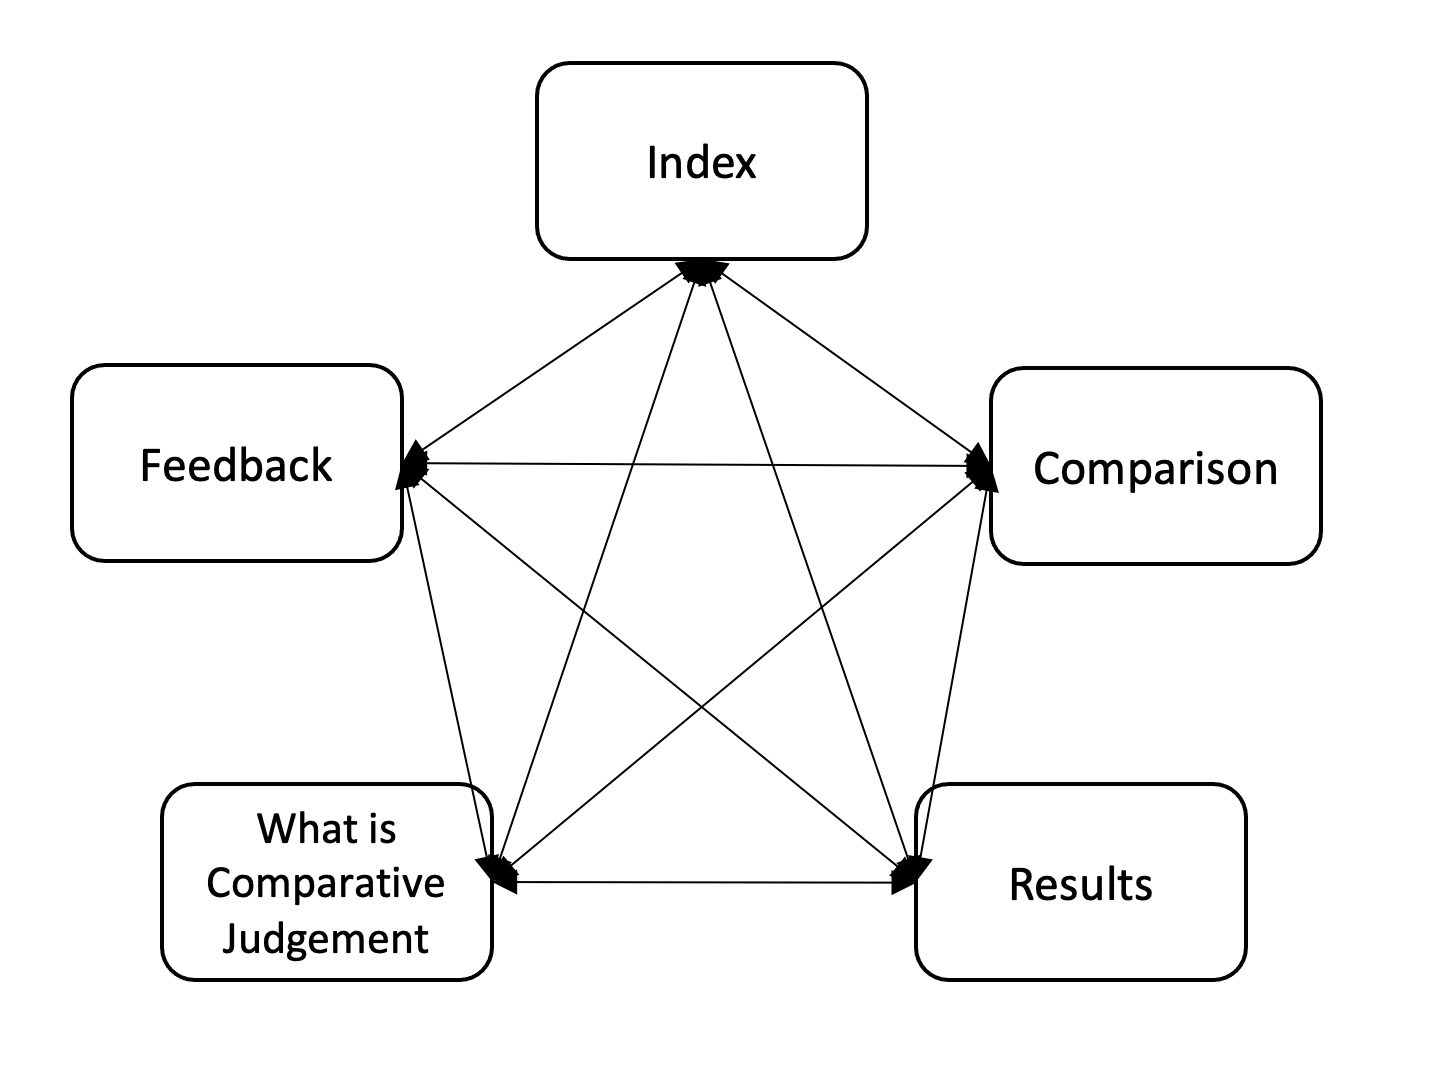
\includegraphics[width=8cm]{web_app_nav.png}
		\caption{A visual representation of the web apps navigation.}
		\label{fig:web_app_nav}
		
	\end{figure}
	
	Additional tools like Google's Firebase was used to handle user authentication and store the web app's content in their real-time databases. The real-time databases are a NoSQL document notation database that updates in real-time. 
	
	A requirement of the app is for the user to be able to create an account. The account sign-up only requires an email and will generate all the additional requirements for the other parts of the app to work in the background. They are linking all the results for these comparisons to the user's ID. At the point of sign-up, a user position within the comparison cycle gets generated, a random selection of tweets to get compared against will be generated. The logic behind the sampling is that a user will only see a single tweet once. Therefore making sure that the user sees these tweets for the first time, every time, making it more of a fair comparison.
	
	Heroku handled the hosting of the web app. Heroku is a free-to-use web hosting provider. However, with it being a free-to-use service, it did bring about some undesirable aspects, mainly the website's slow loading time.
	
	%[Tweet Comparison Presentation]
	As previously mentioned, a user will have a random sample of the tweets, which will have a unique pairing. Therefore ensuring that a user will only see one tweet within the pairing once, to make the tweet's joke not lose its impact as the second or third time a user sees the same tweet, it naturally would lose its edge. Hence, each user will have their own predetermined set of comparisons at the point of sign-up but will one see, for example, tweet one once. As we mentioned, this was to keep the tweets fresh for the user and make them more likely to complete all the comparisons. Otherwise, if the user had to see all unique comparisons, they would have to see 45 different combinations in total just for ten different tweets. So if we put this into the context of a teacher, who would usually have 30 students in a class, several teachers will have to see 435 different combinations, which is just for one class. When this gets factored in, we are looking at around 11175 for 150 different students.
	
	The app will query the database and look for the user's current position when presenting the tweets. Based on their position, the tweet combinations then get checked for that according to the round. The tweet ids are then queried against the tweets' content and then presented to the web page. The user gets expected to select a tweet that they find funnier and then provide an opportunity to justify their choice, which is optional.   
	
	When the user presses the "Vote!" button, this saves the results to the database, updating the two result systems and the user's position. The process will save which tweet won and lost and update the ELO ranking and the standard ranking. The standard ranking gets calculated by taking how many times a tweet has won minus the number it has lost. The implementation of the standard ranking system is to try to implement a more traditional comparative judgement ranking system. In contrast, the ELO system is using a more traditional approach (see fig: \ref{fig:elo_maths}) Which gets updated after every comparison. The implementation of the two systems allows us to see if the ELO or more standard version of CJ is the more effective one or if they naturally mirror each other.
	
	\begin{figure}[t]
		\centering
		$ Prob A Wins = 1/1+10^{(B-A/400)}$
		\caption{To calculate the expected score for a tweet.}
		new score $= rating + 32 * $  score $ - $expected score
		\caption{A visual representation of the web apps navigation.}
		\label{fig:elo_maths}
		
	\end{figure}
	
	This process gets repeated until the user has completed all five comparisons.
	
	\section{Designs}
	
	\subsection{Home Page}
	\subsection{Comparison Page}
	\subsection{What is Comparative Judgement Page}
	\subsection{Results Page}
	\subsection{Feedback Page}
	
	